\chapter{Eigenes Verfahren}
In diesem Kapitel soll das eigene Verfahren beschrieben werden. Es geht dabei nicht nur darum zu beschreiben was gemacht wurde, sondern ebenfalls darum zu begr�nden, weshalb bestimmte Design-Entscheidungen getroffen wurden.


\section{LaTex-Editoren}

Ein guter Cross-Plattform (Windows/Linux/Mac) Latex-Editor mit englischer und deutscher Rechtschreibkorrektur ist z.B. TexStudio
(\url{http://texstudio.sourceforge.net/}). Unter Windows verwende ich diesen Editor gerne zusammen mit dem Sumatra PDF Viewer (\url{http://blog.kowalczyk.info/software/sumatrapdf/free-pdf-reader.html}), da dieser ein automatisches Neuladen unterst�tzt.

%%%%%%%%%%%%%%%%%%%%%%%%%%%%%%%%%%%%%%%%%%%%%%%%%%%%%%%%%%%%%%%%%%%%%%%%%%%%%%%%%%%%%%%%%%%%%%%%%%%%%%%%%%%%%%%%%%%%%%%%%
\section{Beispiel f�r eine Tabelle}
In Tabelle \ref{tab:bibliotheken} sind die verwendeten Bibliotheken ausgelistet.
\begin{table}[htbp]
\centering 
\begin{tabular}{ll}
\toprule \textbf{Bibliothek} & \textbf{Version} \\
\bottomrule
CUDA SDK & 2.3 \\
CUDA Toolkit & 2.3 \\
 OpenGL & 3.2 \\
 GLUT & 3.7 \\
GLEW & 1.5.1 \\
CUDPP & 1.1 \\
\bottomrule
\end{tabular}
\caption{Die verwendeten Bibliotheken.}
\label{tab:bibliotheken}
\end{table}

\section{Formel in Latex und Konventionen zur Verwendung mathematischer Symbole}
Mathematische Symbole k�nnen in Latex sehr leicht erzeugt werden. Beispiel f�r Symbole im Text: Gegeben sei ein Skalar $a \in \mathbb{R}$. Tabelle~\ref{tab:mathematischeSymbole} liste einige Konventionen zur Verwendung mathematischer Symbole. Abgesetzte Formel lassen sich ebenfalls leicht erzeugen:
\begin{equation}
\label{eqn:beispiel}
f(x) = x^2 + 3
\end{equation}
Au�erdem kann leicht auf abgesetzte Formel verwiesen werden (siehe Gleichung~\ref{eqn:beispiel}). F�r mehrere ausgerichtete Formeln bietet sich die Umgebung \texttt{eqnarray} an:
\begin{eqnarray}
\label{eqn:beispiel2}
f(x) &=& x^2 + 3 \\
g(\theta) &=& \cos (2\theta) = \cos^2 \theta - \sin^2 \theta\\
h(x) &=& \int_0^\infty \mathrm{e}^{-x}\,\mathrm{d}x
\end{eqnarray}


\begin{table}[htbp]
\centering
\begin{tabular}{lll}
\toprule \textbf{Typ} & \textbf{Schriftart} & \textbf{Beispiele} \\
\bottomrule
Variablen (Skalare) & kursiv & $a, b, x, y$ \\
Funktionen & aufrecht& $\mathrm{f}, \mathrm{g}(x), \mathrm{max}(x)$\\
Vektoren & fett, Elemente zeilenweise & $\mathbf{a}, \mathbf{b}= \begin{pmatrix}x\\y\end{pmatrix} = (x, y)^\top$\\
Matrizen & Schreibmaschine& $\mathtt{A}, \mathtt{B}= \begin{bmatrix}a & b\\c & d\end{bmatrix}$\\
Mengen & kalligrafisch& $\mathcal{A}, \{a, b\} \in \mathcal{B}$ \\
Zahlenbereiche & doppelt gestrichen& $\mathbb{N}, \mathbb{Z}, \mathbb{R}^2, \mathbb{R}^3$ \\
\bottomrule
\end{tabular}
\caption{Konventionen zur Verwendung mathematischer Symbole}
\label{tab:mathematischeSymbole}
\end{table}






\section{Beispiel f�r eine Vektorgrafik}

Wenn m�glich sollten immer Vektorgrafiken verwendet werden. Rastergrafiken sollten nur dann eingesetzt werden, wenn die Original-Quelle ebenfalls eine Rastergrafik ist. Ein 
Cross-Plattform Editor zur Erstellung von Vektorgrafiken ist z.B. Inkscape:
\url{http://inkscape.org/download/}. Nach der Erstellung in Inkscape sollte die Grafik zum einen zur sp�teren Weiterverarbeitung als SVG gespeichert werden. Zum anderen zwecks Import in Latex als PDF. Abbildung~\ref{fig:vectorExample} zeigt ein Beispiel.


\begin{figure}[htpb]
	\centering
		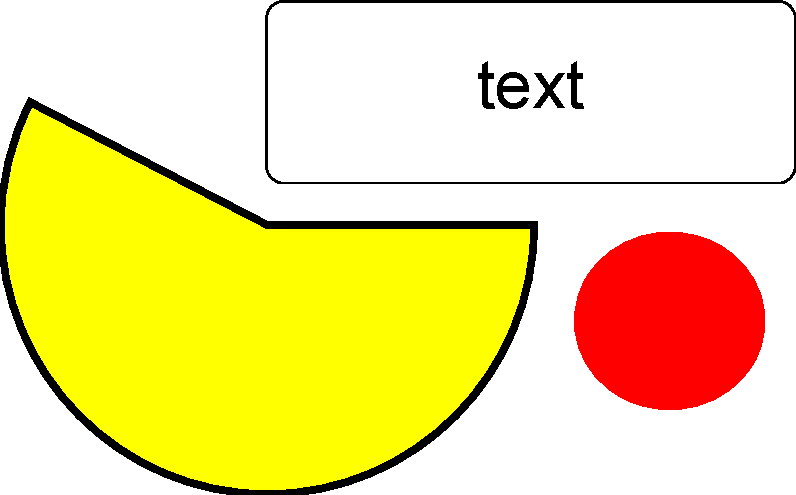
\includegraphics[width=0.30\textwidth]{fig/vectordrawing.pdf}
	\caption{Eine Vektorgrafik}
	\label{fig:vectorExample}
\end{figure}


\section{Beispiel f�r eine Vektorgrafik mit mathematischen Symbolen}

Um beliebigen Latex-Code in eine Vektorgrafik einzuf�gen (z.B. um mathematische Symbole zu setzen) kann in Inkscape beim Speichern der Datei als PDF die Option \glqq Pdf+Latex: Text in PDF weglassen und Latex Datei erstellen\grqq  ~angew�hlt werden (siehe Abb.~\ref{fig:vectorExampleSymbol})

\begin{figure}[htpb]
    \centering
    \def\svgwidth{0.30\textwidth}
  	\import{./fig/}{vectordrawingSymbol.pdf_tex}
	\caption{Eine Vektorgrafik mit mathematischen Symbolen}
	\label{fig:vectorExampleSymbol}
\end{figure}

\section{Beispiel f�r eine Rastergrafik}

Abbildung~\ref{fig:exampleFigure} zeigt, wie eine Rastergrafik eingebunden werden kann. \\

\begin{figure}[htpb]
    \centering
  	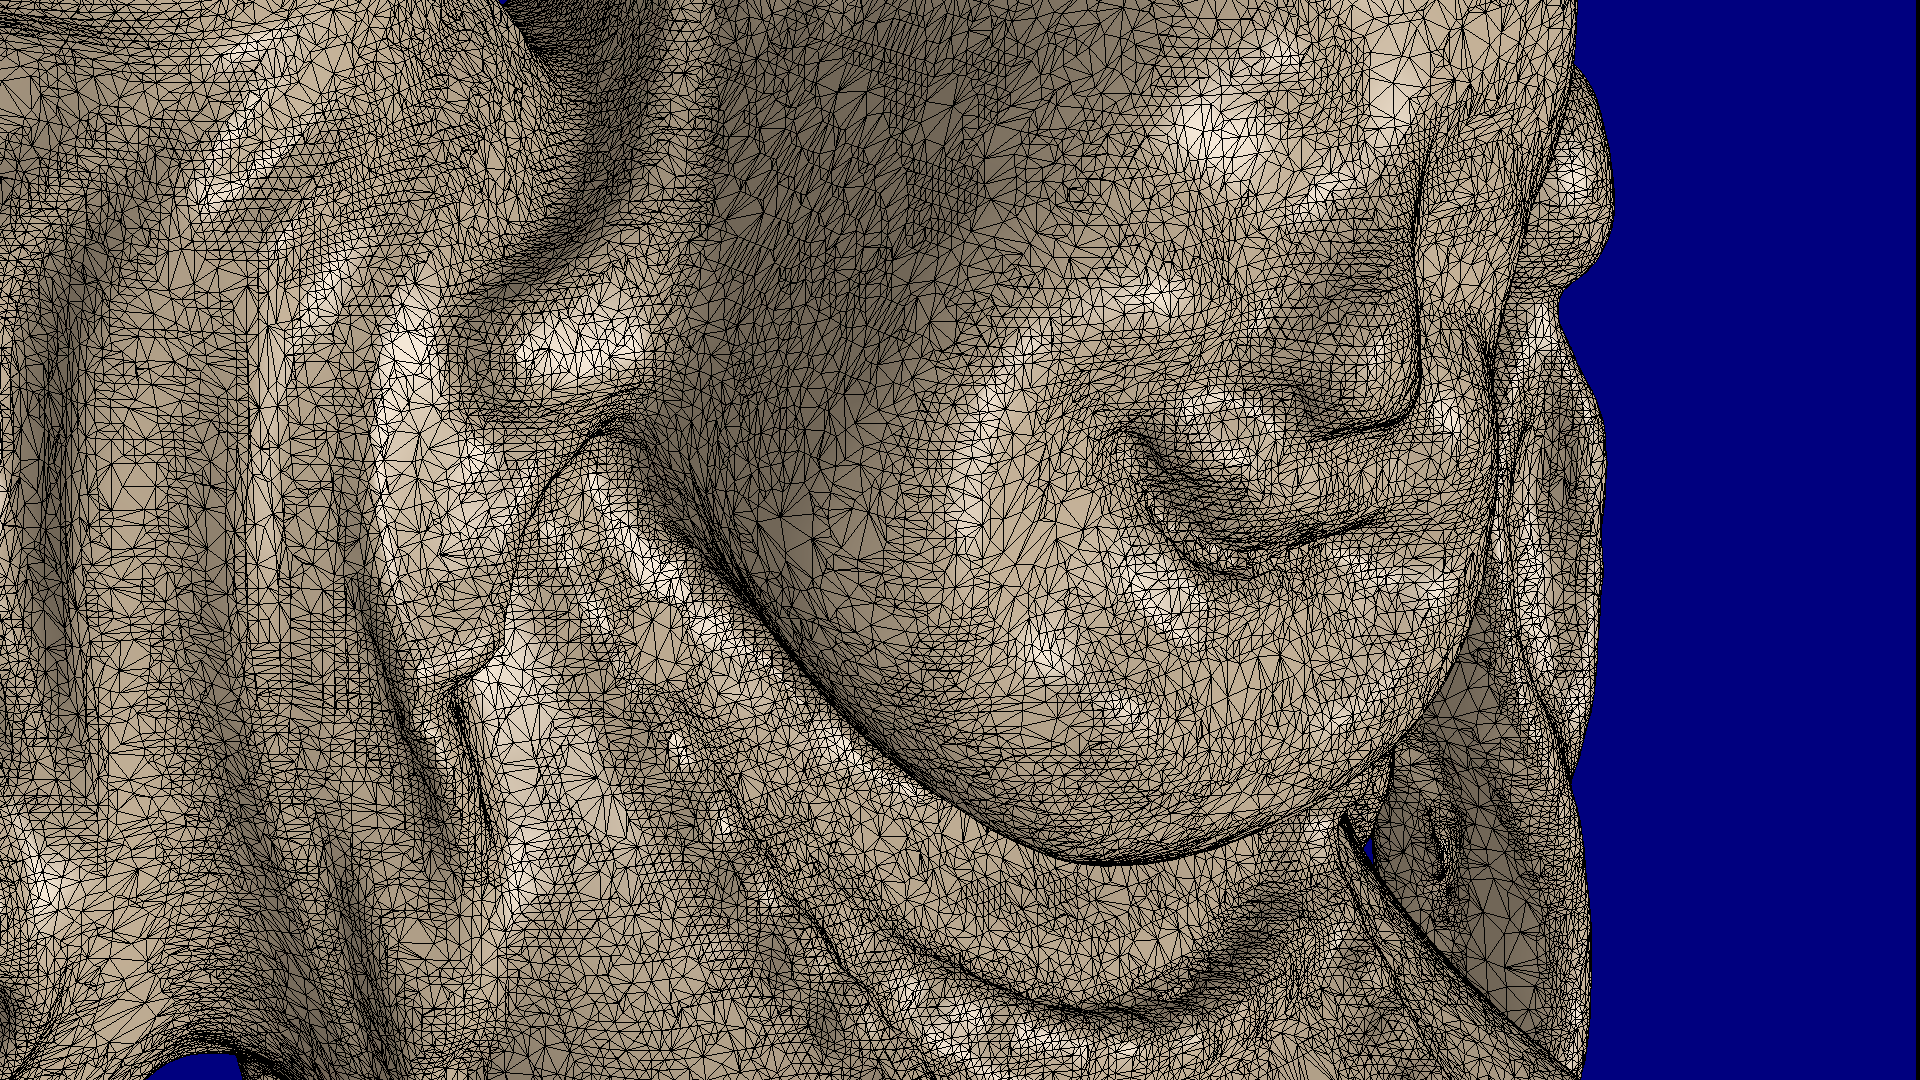
\includegraphics[width=0.80\textwidth]{fig/Buddha2.png}
	\caption{Eine Rastergrafik}
	\label{fig:exampleFigure}
\end{figure}


Bild- bzw. Tabellen-Beschriftungen sollten m�glichst informativ sein. Aus der Beschreibung sollte die Bedeutung der Abbildung vollst�ndig hervorgehen, so dass der Haupttext zum Verst�ndnis nicht notwendigerweise gelesen werden muss. 

\newpage
\section{Beispiel f�r die Darstellung von Algorithmen}

Algorithmus \ref{algo:algorithmSCAN} zeigt ...

\begin{algorithm}[htpb]
	\textit{Phase 1: Reduktion}\\
	\texttt{for} $d := 0$ \texttt{to} $log_2 n - 1$ ~\texttt{in parallel do}\\
	\hspace{5mm}\texttt{for} $k := 0$ \texttt{to} $n - 1$ \texttt{by} $2^{d+1}$ ~\texttt{in parallel do}\\
	\hspace{10mm}$x[k + 2^{d + 1} - 1] := x[k + 2^d - 1] + x [k + 2^{d + 1} - 1]$\\
	\textit{Phase 2: Propagation}\\
	\texttt{for} $d := log_2 n$ \texttt{to} $0$ ~\texttt{in parallel do}\\
	\hspace{5mm}\texttt{for} $k := 0$ \texttt{to} $n - 1$ \texttt{by} $2^{d+1}$ ~\texttt{in parallel do}\\
	\hspace{10mm}$t := x[k + 2^d - 1]$\\
	\hspace{10mm}$x[k + 2^d - 1] := x [k + 2^{d + 1} - 1]$\\
	\hspace{10mm}$x[k + 2^{d + 1} - 1] := t + x [k + 2^{d + 1} - 1]$\\
	\caption{Pseudocode der zwei Phasen vom SCAN-Algorithmus \cite{bib:SCAN}.}
	\label{algo:algorithmSCAN}
\end{algorithm}

\section{Beispiel f�r die Darstellung von Quellcode-Ausz�gen}


Listing \ref{lst:VBOkontrolle} zeigt ...

\begin{lstlisting}[float = htpb,caption={Pseudocode f�r die Kontrolle der VBOs.}, label=lst:VBOkontrolle,captionpos=b,keywordstyle=\bfseries\color{black}] 
void Adapt() {
  cudaGLMapBufferObject( � , vertVbo);
  cudaGLMapBufferObject( � ,  indVbo);
	�
  cudaGLUnmapBufferObject(vertVbo);
  cudaGLUnmapBufferObject( indVbo);
}
\end{lstlisting}

